\documentclass[resume]{subfiles}


\begin{document}
\section{Introduction}
\begin{figure}[H]
\centering
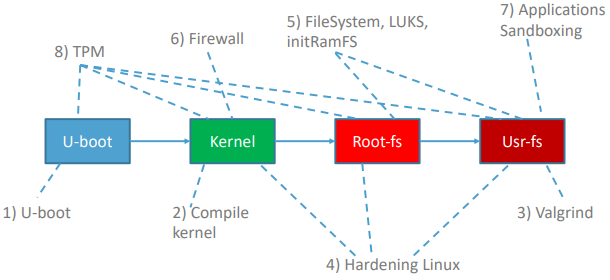
\includegraphics[width=0.8\columnwidth]{img_0.png}
\end{figure}
\paragraph{Attaques de surface}  : Utilisateurs des ports de debug, connecteurs, Alimentations
\paragraph{Vecteurs d'attaque} : Réseau (Ethernet, Wifi), application, port série, USB, I2C, Flash, Bluetooth, GPS, etc...
\subsection{Compilation pour nanopi}
Cross-compilation (ARM) effectuée sur un système x86/x64. Buildroot est le toolchain utilisé. Les éléments suivants sont compilés : Bootloader, Kernel, Rootfs

Puis les images sont copiées sur la carte SD
\end{document}